%!TEX root = ../dokumentation.tex
\section{Funktionsumfang}
Die Aufgabenstellung ist im Kapitel 1 detailiert beschrieben. \\
Es wurde eine Liste mit Funktionen erstellt, die für das erreichen des Projektziel notwendig sind.
\begin{itemize}
    \item Das Script soll täglich mittels Cronjob ausgelöst werden.
    \item Klonen eines Projekt aus GitHub. 
    \item Erstellen einer virtuellen Umgebung mittels virtualenvwrapper.
    \item Installieren des Projekts und deren Abhängigkeiten.
    \item Aufsetzen einer mysql-Datenbank. 
    \item Synchronisieren der Datenbank mit den Djangomodellen.
    \item Ausführen der Datenbankmigrationen.
    \item Überprüfung des Quellcodes anhand der vorgegebenen Validierungskriterien (siehe Abschnitt Validierungskriterien).
    \item Starten der Djangoapplikation
    \item Alle Berichte werden in eine Logdatei geschrieben. 
    \item Senden eines Berichts als Email an eine vordefinierte Adresse.
    \item Entfernen der Datenbank aus der lokalen Umgebung.
    \item Entfernen des überprüften Projekt und der virtuellen Umgebung aus der lokalen Umgebung.
\end{itemize}


\section{Validierungskriterien}
Folgende Kriterien müssen erfüllt sein, damit ein Djangoprojekt erfolgreich validiert wird:
\begin{itemize}
    \item Codeüberprüfung durch pep8 - *.py
    \item Codeüberprüfung durch pyflakes - *.py
    \item Codeüberprüfung durch jshint - *.
    \item Der Code darf die folgenden Zeichenfolgen nicht enthalten: ''console.log'', ''debugger'' - *.js
    \item Der Code darf die folgenden Zeichenfolgen nicht enthalten: ''print'', ''import pdb'', ''import ipdb'' - *.py
\end{itemize}

\section{Kriterien für die Erweiterbarkeit}
Damit das Script auch bequem erweitert werden kann, muss auf ein paar Dinge besonds geachted werden. \\
Darunter gehören eine modulare Aufteilung der einzelnen Prüfungsprozesse und eine Kapselung des Basiscodes. \\
Mit Einhaltung folgender Kriterien sollte das möglich sein:
\begin{itemize}
    \item Die Prüfungsscripts sind in einem separatem Order gespeichert.
    \item Der Bezug auf die Prüfungsscripts wird nur in einer Datei gehalten. 
    \item Das Layout für den Bericht, der über Email versendet wird, wird in einer separaten Datei gehalten.
    \item Der Prüfungsbericht soll so gestaltet sein, dass die Resultate auch bei sehr vielen Projekten oder sehr vielen Prüfungsprozessen noch überschauber ist.
\end{itemize}

\clearpage
\section{Prüfungsbericht}
Der Prüfungsbericht wird nach Abschluss der Überprüfung aller Projekte als Email versendet. Im Bericht sollen alle Diagnosen der Projekte aufgezählt sein.
Der Bericht wird in eine Gesamtsübersicht und in einer Detailübersicht aufgeteilt. Die Gesamtübersicht wird immer angezeigt und stellt alle Projekte und eine grobe Erfolgsanzeige in einer Tabelle dar. \\
Die Detailanzeige wird nur dan angezeigt, wenn bei der Überprüfung eines Projekts Mängel auftauchen. Jedes Projekt, dass die Überprüfung nicht erfolgreich abgeschlossen hat, bekommt seine eingen Detailansicht.
In der Detailansicht wird jediglich darauf hingewiesen, welcher Prüfungsprozess einen Fehler zurückgibt. Die originale Fehlermeldung wird nicht angezeigt. 

\section{Modulstruktur des Scripts}
Wie bereits in dem Abschnit ''Kriterien für die Erweiterbarkeit'' erwähnt, soll das Script mit Prüfungsprozessen erweiterbar sein ohne den Basiscode zu verändern. Im folgenden Abschnitt wird genauer auf die Aufteilung der einzelnen Module eingegangen. \\

\section{Scriptablauf}
\subsection{Abarbeitung der Djangoprojekt}
Es werden alles Djangoprojekt nacheinander überprüft. Am schluss wird der Bericht per Mail versendet.
Im nachfolgendem Flussdiagramm ist ersichtlich, wie die Projekte nacheinander abgearbeited werden: \\

\begin{center}
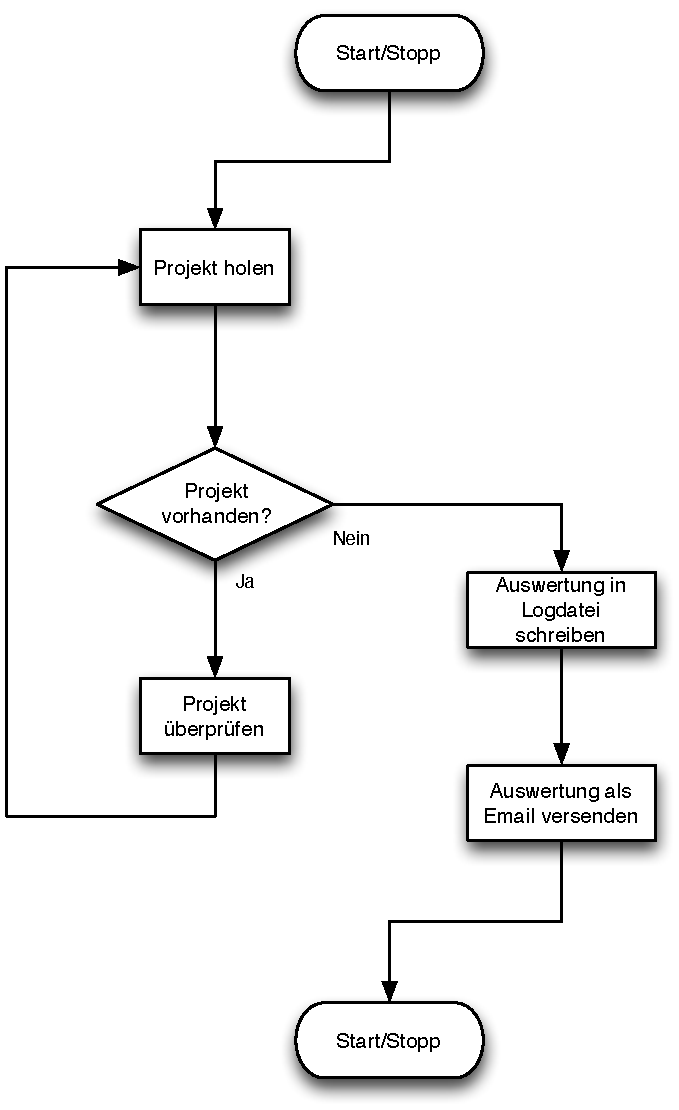
\includegraphics[width=0.6\textwidth,angle=0]{./grafiken/pzd_projektabarbeitung.pdf}
\end{center}

\subsection{Arbeitsablauf der Testcases in einem Djangoprojekt}
Die Testcases werden nacheinander geladen und aufgerufen. Nach jedem abgeschlossenen Testcase wird das entsprechnde Resultat für die Auswertung zwischengespeichert. 
Die Überprüfung eines Djangoprojekts ist abgeschlossen, wenn alle Testfälle durchgelaufen sind oder ein Testfall gescheitert ist, welcher als erfolgsabhängig eingestuft wurde. 
Im nachfolgendem Flussdiagramm ist ersichtlich, wie die Testcases in einem Projekt nacheinander abgearbeited werden: \\ 

\begin{center}
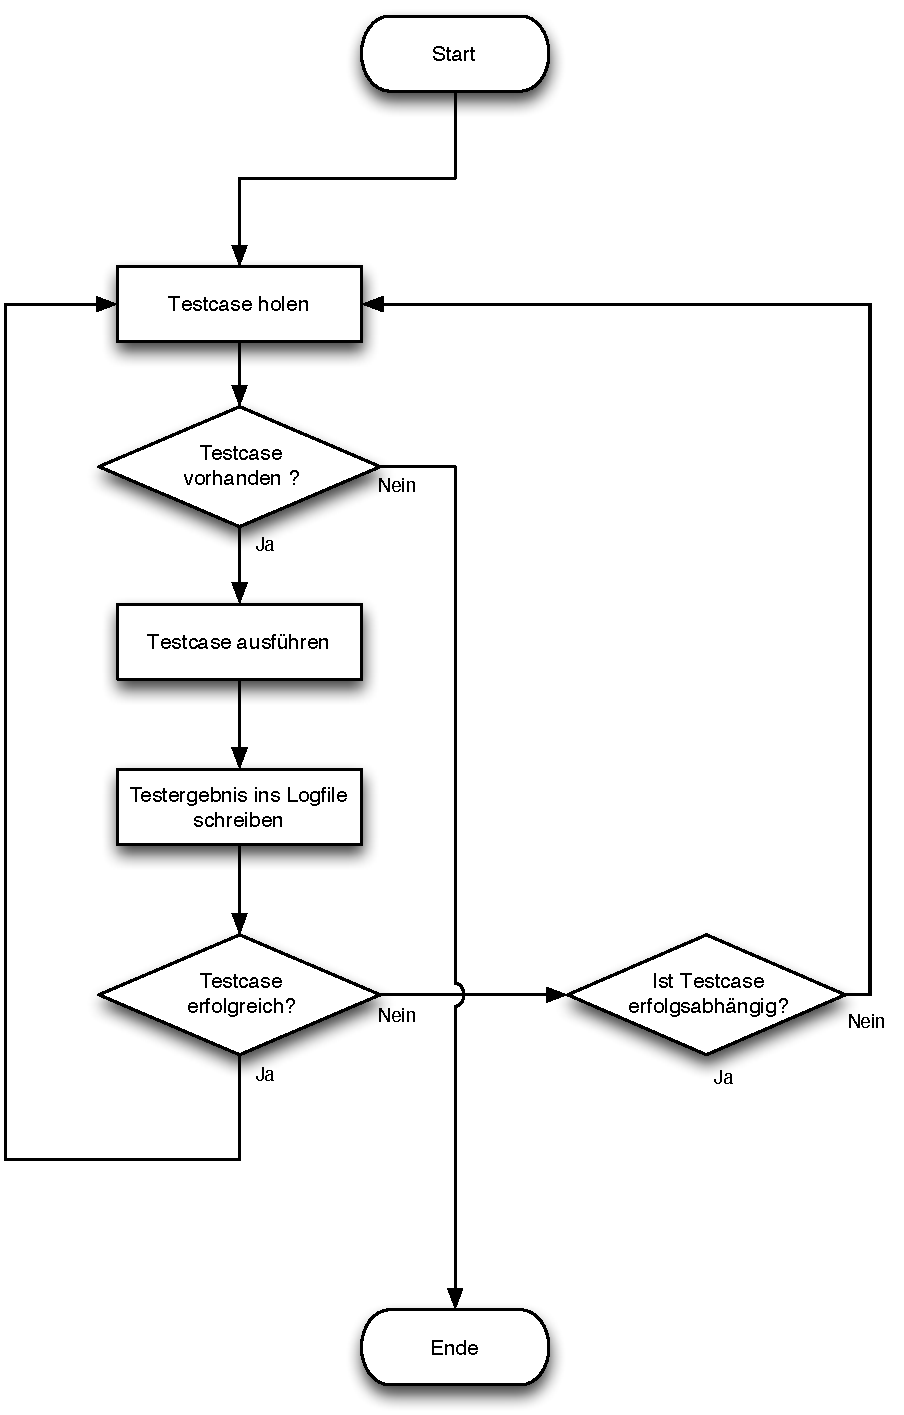
\includegraphics[width=0.8\textwidth,angle=0]{./grafiken/pzd_djangoprojekt.pdf}
\end{center}

\clearpage
